
\chapter{METODOLOGI PENELITIAN}
\label{cha:3-MetodologiPenelitian}

\section{Gambaran Umum} \label{sec:3-GambaranUmum}

Penelitian ini membahas pemanfaatan data gambar sebagai acuan dalam melakukan pemelajaran dan
implementasi model \textit{deep neural network} untuk mencari dan memetakan koordinat tiga dimensi
pose tubuh manusia dalam sebuah rangkaian gambar secara lokal.
Pose yang digunakan tidak bersifat \textit{grounded} yang berarti koordinat pose tidak berpusat pada
titik lantai tertentu.
Pengerjaan aplikasi mengutamakan dua
langkah penting yang meliputi pengolahan data dan pembuatan model. Aplikasi yang dibuat dapat menampilkan
plot grafik tiga dimensi menyerupai struktur anatomi tubuh manusia sesuai dengan pose hasil
estimasi dari gambar masukkan.
Hasil pemelajaran model ditampilkan dalam grafik dua dimensi untuk analisis lebih lanjut.

\textit{Dataset} yang digunakan dalam penelitian ini terbagi menjadi dua jenis yang meliputi
\textit{dataset} pemelajaran model dan \textit{dataset} inferensi aplikasi.
\textit{Dataset} pemelajaran model dikategorikan menjadi data pelatihan model dan data validasi model.
\textit{Dataset} pemelajaran model berisi gambar dan target posisi titik kunci anatomi dalam jumlah besar.
Data pelatihan model adalah data yang digunakan dalam proses pelatihan sebagai sampel bagi \textit{deep neural network}.
Data validasi model adalah data yang digunakan untuk menguji kebenaran fungsionalitas pemetaan yang
dipelajari saat pelatihan model. \textit{Dataset} inferensi aplikasi adalah data uji coba berbentuk
video tanpa target titik kunci yang digunakan untuk estimasi pose tubuh manusia secara sekuensial.

Pemelajaran model \textit{deep neural network} diimplementasikan menggunakan \textit{framework} PyTorch.
Kedua \textit{dataset} yang digunakan diolah terlebih dahulu sehingga memenuhi syarat PyTorch dalam melakukan
\textit{deep learning}.
Setiap model kemudian digunakan terhadap \textit{dataset} inferensi
aplikasi. Proses dan hasil estimasi diurai lebih lanjut dalam bentuk grafik visual.

\section{Kerangka Penelitian} \label{sec:3-KerangkaPenelitian}

Kerangka penelitian yang jelas dibutuhkan untuk memudahkan proses penelitian sehingga dapat
mempersingkat waktu pengerjaan. Proses penelitian dibagi menjadi tiga tahapan besar yang meliputi
tahap praproduksi, tahap produksi, dan tahap uji coba. Setiap tahapan tersebut dikerjakan secara
terurut dan sistematis. Alur setiap tahap diilustrasikan pada gambar~\ref{fig:kerangkapenelitian}.

\begin{figure}[htbp]
    \begin{center}
        \fbox{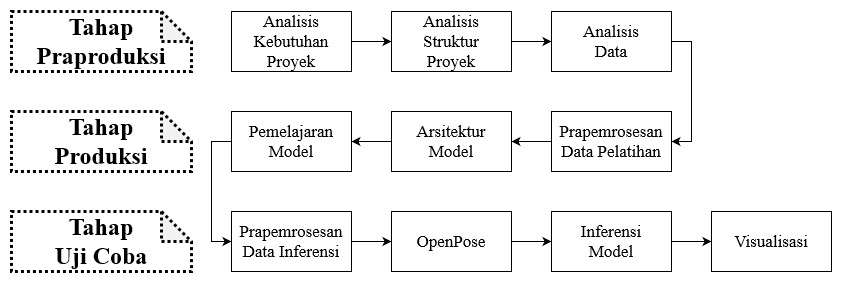
\includegraphics[width=11.9cm]{bab3/gambar/kerangka_penelitian.jpg}}
    \end{center}
    \vspace{-20pt}
    \captionsetup{labelfont=bf, textfont=bf}
    \caption{Kerangka Penelitian}
    \vspace{-10pt}
    \captionsetup{labelfont=md, textfont=md}
    % \caption*{Sumber: sumber}
    % \caption*{Sumber: nama(2019)}
    \label{fig:kerangkapenelitian}
\end{figure}

\section{Tahap Praproduksi} \label{sec:3-TahapPraproduksi}

Tahap praproduksi berisi langkah-langkah analisis yang menentukan alur pada tahap selanjutnya. Tahap
praproduksi dibagi menjadi beberapa langkah yang meliputi analisis kebutuhan proyek, analisis
struktur proyek, dan analisis data. Tahap ini menganalisis bagian-bagian pokok yang diperlukan
sehingga mengetahui langkah-langkah yang akan dilakukan pada tahap produksi.

\subsection{Analisis Kebutuhan Proyek}

Pemelajaran dan implementasi model ini memerlukan alat-alat pendukung berupa perangkat keras dan
perangkat lunak yang mencukupi. Spesifikasi perangkat keras dan perangkat lunak yang lebih besar
akan mempercepat proses pemelajaran model jaringan saraf tiruan.

Spesifikasi perangkat keras yang digunakan dalam penelitian ini meliputi \textit{central processing unit}, \textit{graphics processing unit},
\textit{random access memory}, \textit{solid state drive}, dan \textit{hard disk drive}
dapat dilihat pada tabel~\ref{tab:spesifikasiperangkatkeras}.

\pagebreak

\begin{table}[htbp]
    \captionsetup{labelfont=bf, textfont=bf}
    \caption{Spesifikasi Perangkat Keras}
    \label{tab:spesifikasiperangkatkeras}
    \vspace{-20pt}
    \begin{center}
        \begin{tabular}{|c|c|}
            \hline
            \multicolumn{2}{|c|}{\textbf{Perangkat Keras (Laptop)}} \\ \hline
            CPU & Intel Core I7 7700 HQ                             \\ \hline
            GPU & NVIDIA GTX 1060 6 GB                              \\ \hline
            RAM & 24 GB DDR4                                        \\ \hline
            SSD & NVME SAMSUNG 120 GB                               \\ \hline
            HDD & SATA 1 TB                                         \\ \hline
            % \multicolumn{1}{|c|}{RDF-3X}    & a & b & c & d & e & f & g \\ \hline
        \end{tabular}
    \end{center}
\end{table}


Spesifikasi perangkat lunak yang digunakan dalam penelitian ini yang meliputi sistem operasi,
\textit{integrated development environment}, bahasa pemrograman, dan \textit{deep learning framework}
dapat dilihat pada tabel~\ref{tab:spesifikasiperangkatlunak}.


\begin{table}[htbp]
    \captionsetup{labelfont=bf, textfont=bf}
    \caption{Spesifikasi Perangkat Lunak}
    \label{tab:spesifikasiperangkatlunak}
    \vspace{-20pt}
    \begin{center}
        \begin{tabular}{|c|c|}
            \hline
            \multicolumn{2}{|c|}{\textbf{Perangkat Lunak}} \\ \hline
            Sistem Operasi      & Ubuntu 19.10             \\ \hline
            IDE                 & Jupyter Lab              \\ \hline
            Bahasa Pemrograman  & Python 3.7               \\ \hline
            \textit{Framework } & PyTorch 1.4              \\ \hline
        \end{tabular}
    \end{center}
\end{table}

\subsection{Analisis Struktur Proyek}

Perancangan struktur proyek yang sistematis diperlukan untuk meminimalisir kompleksitas dalam
melakukan pembuatan dan pemelajaran model. \textit{Integrated development environment} Jupyter Lab
memudahkan eksekusi perintah dengan sintaks bahasa pemrograman Python dalam bentuk sel interaktif
dalam berkas berekstensi ipynb. Setiap sel terdiri dari
\textit{input} dan \textit{output}. \textit{Input} berisi perintah yang akan dieksekusi, sedangkan
\textit{output} berisi hasil eksekusi yang dapat berupa teks ataupun grafik. Tampilan Jupyter Lab
dapat dilihat pada gambar~\ref{fig:jupyterlab}.

\begin{figure}[htbp]
    \begin{center}
        \fbox{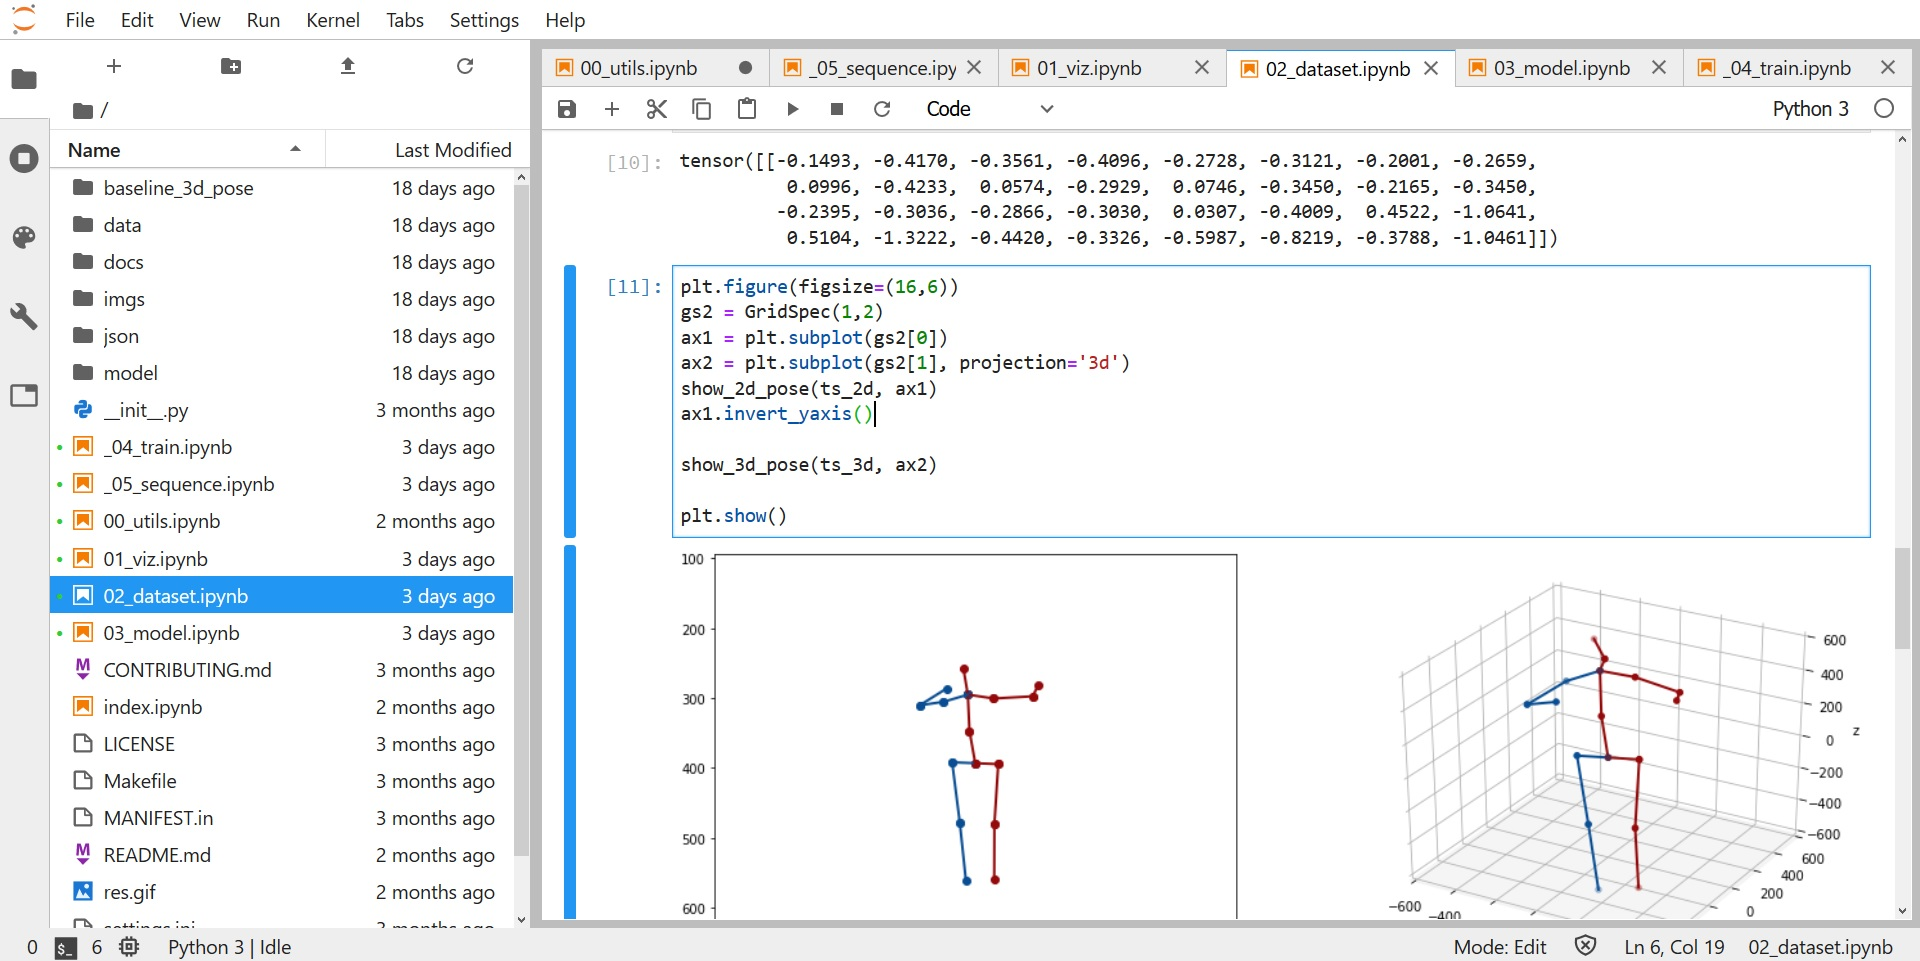
\includegraphics[width=11.9cm]{bab3/gambar/jupyterlab.jpg}}
    \end{center}
    \vspace{-20pt}
    \captionsetup{labelfont=bf, textfont=bf}
    \caption{Jupyter Lab}
    \vspace{-10pt}
    \captionsetup{labelfont=md, textfont=md}
    % \caption*{Sumber: sumber}
    % \caption*{Sumber: nama(2019)}
    \label{fig:jupyterlab}
\end{figure}


Struktur direktori yang disusun terdiri dari empat folder dan enam berkas \textit{interactive python notebook}
berekstensi ipynb. Folder data berisi data latihan model seperti pada gambar~\ref{fig:strukturdirektori}.
Folder imgs berisi rangkaian gambar yang
diambil dari rekaman video. Folder json menampung berkas yang berisi informasi titik kunci dua dimensi saat
inferensi. Folder model berisi \textit{checkpoint} model selama pelatihan.

Berkas berekstensi ipynb berisi kode pemrograman yang dibagi menjadi enam modul.
Berkas 00\_utils merupakan modul utilitas yang memudahkan proses memuat data, menampilkan data, menyimpan data, dan memanipulasi data.
Berkas 01\_viz adalah modul percobaan menampilkan data pelatihan dan data inferensi.
Berkas 03\_model merupakan modul pendefinisian arsitektur model.
Berkas 04\_train adalah modul pelatihan model.
Berkas 05\_sequence adalah modul percobaan inferensi model terhadap rangkaian gambar.

\begin{figure}[htbp]
    \begin{center}
        \fbox{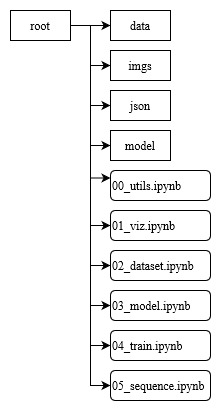
\includegraphics[height=9cm, width=11.9cm]{bab3/gambar/struktur_direktori.jpg}}
    \end{center}
    \vspace{-20pt}
    \captionsetup{labelfont=bf, textfont=bf}
    \caption{Struktur Direktori}
    \vspace{-10pt}
    \captionsetup{labelfont=md, textfont=md}
    % \caption*{Sumber: sumber}
    % \caption*{Sumber: nama(2019)}
    \label{fig:strukturdirektori}
\end{figure}


\subsection{Analisis Data}

Data pembuatan model yang digunakan adalah data pemetaan dari pose dua dimensi ke pose tiga dimensi.
Pose dua dimensi merupakan sampel, sedangkan pose tiga dimensi merupakan target. Sumber data adalah
Human3.6M Dataset mengenai informasi perakaman gerakan pose manusia yang menyimpan gambar dari
beberapa sisi beserta dengan pose dua dimensi dan tiga dimensinya. Informasi kedua pose tersebut
kemudian dipisah dan disimpan dalam file berekstensi "pt"~\cite{h36m_pami}.
Informasi mengenai data pemelajaran dapat dilihat pada tabel~\ref{tab:datapelatihanmodel}.

\begin{table}[htbp]
    \captionsetup{labelfont=bf, textfont=bf}
    \caption{Data Pemelajaran Model}
    \label{tab:datapelatihanmodel}
    \vspace{-20pt}
    \begin{center}
        \begin{tabular}{|c|c|}
            \hline
            Nama Berkas  & Isi                                                                                 \\ \hline
            rcams.pt     & matriks kamera \textit{motion capture} terhadap kamera perekam                      \\ \hline
            stat\_2d.pt  & \textit{mean}, \textit{standard-deviation}, dan \textit{skeleton} pose dua dimensi  \\ \hline
            stat\_3d.pt  & \textit{mean}, \textit{standard-deviation}, dan \textit{skeleton} pose tiga dimensi \\ \hline
            test\_2d.pt  & data pose dua dimensi untuk validasi model                                          \\ \hline
            test\_3d.pt  & data pose tiga dimensi untuk validasi model                                         \\ \hline
            train\_2d.pt & data pose dua dimensi untuk pelatihan model                                         \\ \hline
            train\_3d.pt & data pose tiga dimensi untuk pelatihan model                                        \\ \hline
        \end{tabular}
    \end{center}
    \vspace{-10pt}
\end{table}

Data inferensi model yang digunakan berupa video yang direkam menggunakan kamera diatas sebuah
\textit{tripod}. Hasil rekaman berupa sebuah video monokuler berisi seorang peraga yang memperagakan
berbagai pose dasar. Pose-pose yang diperagakan mencakupi gerakan lengan, gerakan kaki, gerakan pinggang,
gerakan kepala, dan gerakan memutar. Kompleksitas gerakan ini mengakibatkan terjadinya oklusi pada
beberapa bagian badan yang berarti suatu anggota badan menutupi anggota badan lainnya.

Kualitas perekaman video diturunkan dengan menggunakan pencahayaan yang satu arah.
Efek \textit{motion blur} diaktifkan sehingga gerakan yang cepat akan mengalami pengaburan.
Kompleksitas gambar juga ditingkatkan dengan
\textit{aspect ratio} yang bernilai 19 : 6 dengan tipe rekaman \textit{potrait} menyebabkan area rekaman
hanya berada ditengah dan diapit oleh area piksel hitam.

% TODO: disni
\textit{Frame} 00077

% Beberapa \textit{frame} dari data inferensi model dapat dilihat pada gambar
% ~\ref{fig:frame00077},~\ref{fig:frame00173}, dan~\ref{fig:frame00232}.

\begin{figure}[htbp]
    \begin{center}
        \fbox{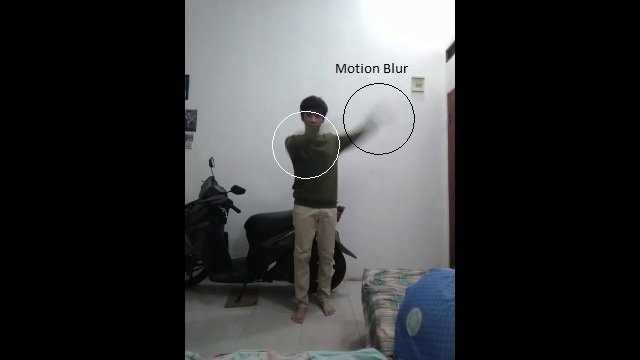
\includegraphics[width=11.9cm]{bab3/gambar/00077.jpg}}
    \end{center}
    \vspace{-20pt}
    \captionsetup{labelfont=bf, textfont=bf}
    \caption{\textit{Frame} 00077}
    \vspace{-10pt}
    \captionsetup{labelfont=md, textfont=md}
    % \caption*{Sumber: sumber}
    % \caption*{Sumber: nama(2019)}
    \label{fig:frame00077}
\end{figure}

\begin{figure}[htbp]
    \begin{center}
        \fbox{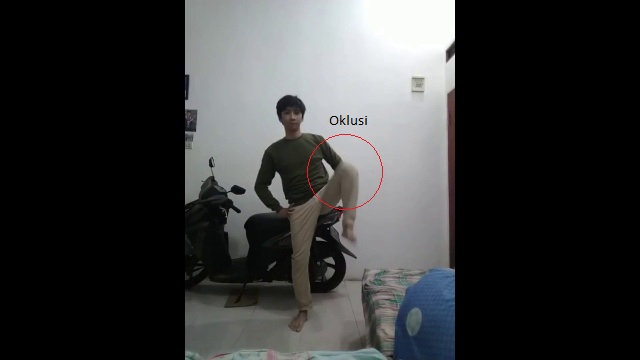
\includegraphics[width=11.9cm]{bab3/gambar/00173.jpg}}
    \end{center}
    \vspace{-20pt}
    \captionsetup{labelfont=bf, textfont=bf}
    \caption{\textit{Frame} 00173}
    \vspace{-10pt}
    \captionsetup{labelfont=md, textfont=md}
    % \caption*{Sumber: sumber}
    % \caption*{Sumber: nama(2019)}
    \label{fig:frame00173}
\end{figure}

\begin{figure}[htbp]
    \begin{center}
        \fbox{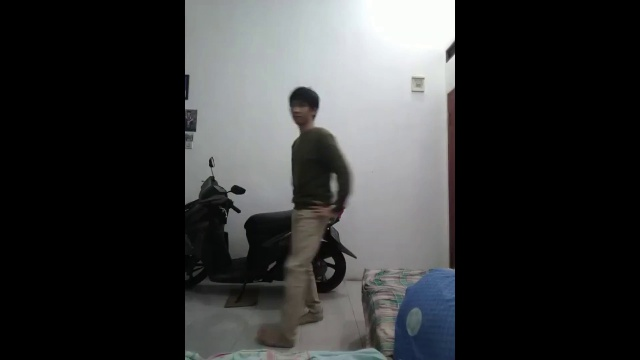
\includegraphics[width=11.9cm]{bab3/gambar/00232.jpg}}
    \end{center}
    \vspace{-20pt}
    \captionsetup{labelfont=bf, textfont=bf}
    \caption{\textit{Frame} 00232}
    \vspace{-10pt}
    \captionsetup{labelfont=md, textfont=md}
    % \caption*{Sumber: sumber}
    % \caption*{Sumber: nama(2019)}
    \label{fig:frame00232}
\end{figure}

\section{Tahap Produksi} \label{sec:3-TahapProduksi}

Tahap produksi merupakan tahap kedua yang dimana pengerjaan dilakukan. Tahap ini terdiri dari
tiga langkah utama yaitu prapemrosesan data pelatihan, pembuatan arsitektur model, dan pemelajaran model.


\subsection{Prapemrosesan Data Pelatihan}

\textit{Dataset} pembuatan model terbagi menjadi dua kategori yaitu data pelatihan
(train\_2d.pt dan train\_3d.pt) dan data validasi (test\_2d.pt dan test\_3d.pt) .
Kedua data ini memiliki struktur dan bentuk yang sama sehingga prapemrosesan yang dilakukan juga sama.
Setiap sampel pada data terdiri dari satu pose dua dimensi dan satu pose tiga dimensi.
Perbedaan daripada kedua data ini terletak pada jumlah sampelnya. Data pelatihan berisi sebanyak
1.559.752 pasang sampel sedangkan data validasi memiliki 550.644 pasang sampel.

Berkas test\_2d.pt, test\_3d.pt, train\_2d.pt, dan train\_3d.pt merupakan berkas hasil konversi
struktur data \textit{dictionary} yang telah berbentuk \textit{serialized}.
Struktur \textit{dictionary} yang berada didalam memori disimpan ke media SSD dalam bentuk \textit{byte stream}.
Berkas-berkas ini harus dibaca dengan mekanisme \textit{deserializing} yaitu membangun ulang sebuah
struktur data yang sama dengan membaca rangkaian \textit{byte} sehingga dapat digunakan pada proses pelatihan model.

Mekanisme pemuatan data dilakukan secara \textit{stochastic} dikarenakan hasil konversi data yang
berukuran sangat besar. Serangkaian pasangan kunci dan target diproses dengan ukuran tertentu
yang disebut dengan \textit{mini-batch} sehingga
VRAM pada GPU tidak mengalami \textit{overflow}. Pemuatan data secara \textit{stochastic} juga
mempercepat proses pelatihan model karena lebih sedikit data yang harus dikalkukasi sebelum melakukan
pemuktahiran.

Kelas Dataset dan DataLoader pada \textit{framework} PyTorch memiliki fungsionalitas untuk melakukan
pembacaan dan pembagian rangkaian data secara \textit{stochastic}. Kelas Dataset dapat membaca berkas
berekstensi "pt" dari media SSD kemudian dimuat kedalam memori. Kelas DataLoader dapat memindahkan
informasi didalam kelas Dataset ke VRAM pada GPU berbentuk \textit{mini-batch} sehingga dapat diproses secara
\textit{stochastic} dan paralel.

Prapemrosesan data pelatihan dan data validasi dilakukan dengan cara yang sama. Langkah pertama
yang dilakukan adalah melakukan cek apakah data yang diinginkan adalah data pelatihan atau data
validasi. Data tersebut kemudian dimuat dan disimpan kedalam memori. DataLoader menerima objek
tersebut kemudian melakukan pengacakan data dan pembagian \textit{mini-batch}. Hasil objek dapat
diiterasi untuk melakukan pelatihan model. Skema prapemrosesan data dapat dilihat pada gambar~\ref{fig:act_diagram}.

\begin{figure}[htbp]
    \begin{center}
        \fbox{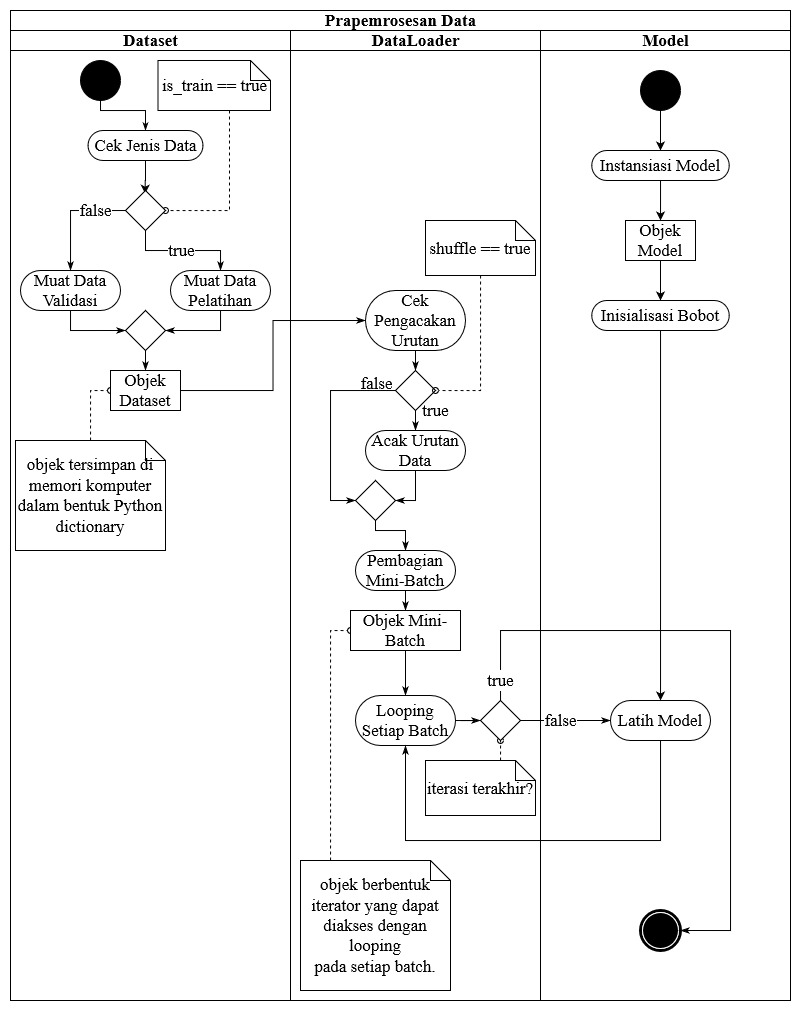
\includegraphics[width=11.9cm]{bab3/gambar/act_diagram.jpg}}
    \end{center}
    \vspace{-20pt}
    \captionsetup{labelfont=bf, textfont=bf}
    \caption{\textit{Activity Diagram} Prapemrosesan Data}
    \vspace{-10pt}
    \captionsetup{labelfont=md, textfont=md}
    % \caption*{Sumber: sumber}
    % \caption*{Sumber: nama(2019)}
    \label{fig:act_diagram}
\end{figure}

\subsection{Arsitektur Model}

Arsitektur model jaringan saraf tiruan yang digunakan memiliki \textit{input} berbentuk vektor dengan ukuran
tiga puluh dua dan \textit{output} berbentuk vektor dengan ukuran empat puluh delapan. Rangkaian lapisan yang
menghubungkan \textit{input} dan \textit{output} berupa lapisan \textit{residual network}. Bobot setiap
lapisan diinisialisasi secara acak dengan distribusi normal.

Sebuah lapisan \textit{residual network} merupakan jaringan dengan arsitektur kecil dan sederhana yang
dapat dipasang atau dibongkar secara modular yang disebut ResLinear. Lapisan ResLinear melakukan operasi
penjumlahan antara \textit{input} dan \textit{output}. Sebuah ResLinear memiliki dua
lapisan linier, dua lapisan \textit{Batchnorm}, dua lapisan \textit{Dropout}, dan dua lapisan \textit{ReLU}.
Komponen-komponen penyusun sebuah lapisan ResLinear dengan ukuran \textit{input a} dan ukuran \textit{output b} seperti
pada gambar~\ref{fig:reslinear}.

\begin{figure}[htbp]
    \begin{center}
        \fbox{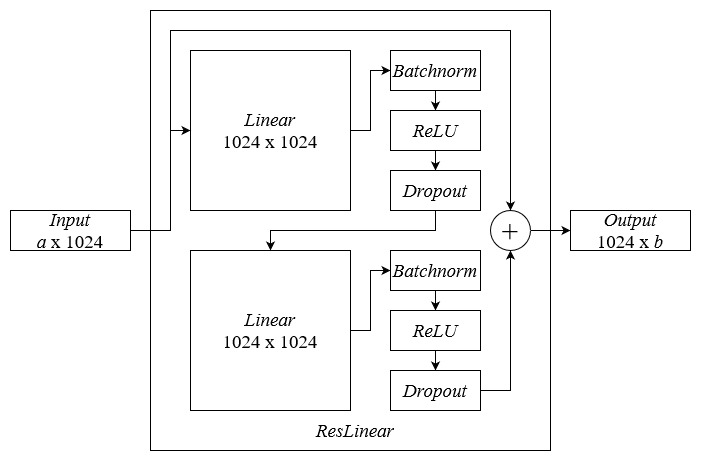
\includegraphics[width=11.9cm]{bab3/gambar/reslinear.jpg}}
    \end{center}
    \vspace{-20pt}
    \captionsetup{labelfont=bf, textfont=bf}
    \caption{Arsitektur Lapisan ResLinear}
    \vspace{-10pt}
    \captionsetup{labelfont=md, textfont=md}
    % \caption*{Sumber: sumber}
    % \caption*{Sumber: nama(2019)}
    \label{fig:reslinear}
\end{figure}

Arsitektur model secara keseluruhan terdiri dari tiga kelompok yang meliputi lapisan awal, lapisan
\textit{residual}, dan lapisan akhir. Lapisan awal menjembatani data \textit{input} dan lapisan \textit{residual}
dengan menggunakan sebuah lapisan linier sebagai penyambung. Lapisan \textit{residual} terdiri dari
dua buah lapisan ResLinear yang berfungsi untuk memetakan pola data \textit{input} terhadap data \textit{output}.
Lapisan akhir menjembatani hasil pemetaan yang dilakukan oleh lapisan \textit{residual} terhadap data \textit{output}.
Arsitektur model dapat dilihat pada gambar~\ref{fig:arsitektur}.

\begin{figure}[htbp]
    \begin{center}
        \fbox{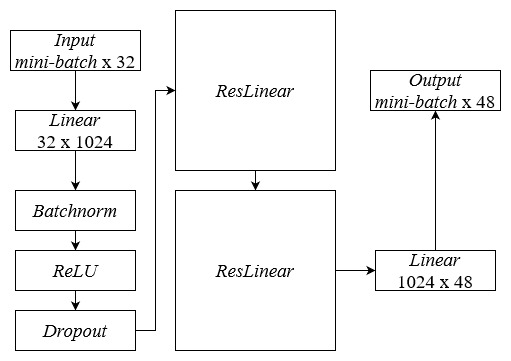
\includegraphics[width=11.9cm]{bab3/gambar/arsitektur.jpg}}
    \end{center}
    \vspace{-20pt}
    \captionsetup{labelfont=bf, textfont=bf}
    \caption{Arsitektur Model}
    \vspace{-10pt}
    \captionsetup{labelfont=md, textfont=md}
    % \caption*{Sumber: sumber}
    % \caption*{Sumber: nama(2019)}
    \label{fig:arsitektur}
\end{figure}

\subsection{Pemelajaran Model}

Pemelajaran model merupakan kelanjutan dari prapemrosesan data. Sebuah model baru diinstansiasii
sehingga menghasilkan objek model. Objek model tersebut kemudian menginisialisasi bobot parameter
dengan bilangan acak dari distribusi normal. \textit{Batch input} yang berasal dari interasi DataLoader
diproses oleh model dengan metode \textit{feed-forward}. Hasil prediksi sementara dari model
didapatkan yang kemudian dibandingkan tingkat kebenarannya menggunakan fungsi kesalahan.
Fungsi kesalahan \textit{mean squared error} menghasilkan angka kuantitas kesalahan. Angka ini merupakan
tolak ukur seberapa akurat kemampuan model dalam menghasilkan output yang relevan. Apabila model tidak
berada dalam status "is\_train", maka kuantitas kesalahan yang didapatkan langsung disimpan dalam bentuk
\textit{array} untuk keperluan analisis. Apabila model berada dalam status "is\_train", maka model
melakukan \textit{backpropagation} untuk menghasilkan gradien bobot. \textit{Learning rate} kemudian
dibagi dengan dua sehingga menjadi lebih kecil. Penyesuaian bobot dilakukan dengan menjumlahkan bobot
dengan hasil operasi perkalian antara \textit{learning rate} dan gradien bobot. Bobot model yang telah
diperbarui disimpan berserta dengan kuantitas kesalahannya. Algoritma yang sama akan diulangi pada setiap \textit{batch input}.
Skema pemelajaran model dapat dilihat pada gambar~\ref{fig:learning}.

\begin{figure}[htbp]
    \begin{center}
        \fbox{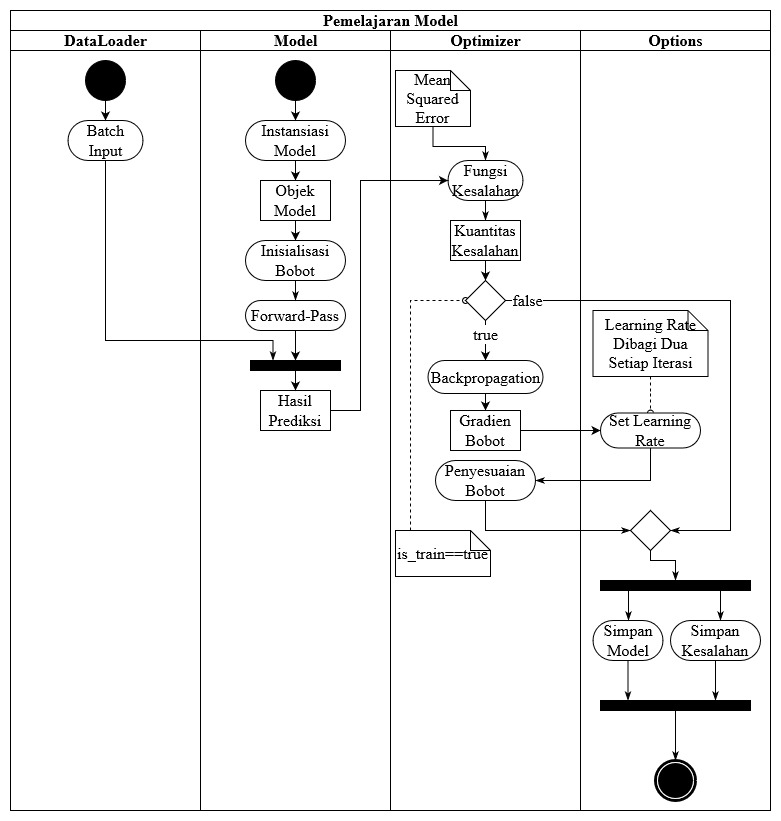
\includegraphics[width=11.9cm]{bab3/gambar/learning.jpg}}
    \end{center}
    \vspace{-20pt}
    \captionsetup{labelfont=bf, textfont=bf}
    \caption{\textit{Activity Diagram} Pemelajaran Model}
    \vspace{-10pt}
    \captionsetup{labelfont=md, textfont=md}
    % \caption*{Sumber: sumber}
    % \caption*{Sumber: nama(2019)}
    \label{fig:learning}
\end{figure}

\section{Tahap Uji Coba} \label{sec:3-TahapUjiCoba}

Tahap uji coba berisi langkah-langkah uji coba penggunaan model.
Tahap uji coba dibagi menjadi beberapa langkah yang meliputi prapemrosesan data inferensi,
penggunaan OpenPose, inferensi model, dan visualisasi. Tahap ini bertujuan untuk menggunakan model
sebagai aplikasi untuk mengestimasi pose tiga dimensi dari gambar monokuler.

\subsection{Prapemrosesan Data Inferensi}

Proses inferensi pose dua dimensi menjadi lebih cepat ketika gambar dua dimensi yang dioperasikan
memiliki resolusi yang kecil. Tingkat resolusi yang digunakan saat merekam pose adalah 640 x 360.
Memperkecil ukuran resolusi juga harus dilihat dari segi kualitas gambar yang dihasilkan.
Gambar juga memiliki banyak informasi statis seperti pada area piksel berwarna hitam yang berada
di kiri dan kanan gambar. Resolusi 290 x 290 dengan titik tengah berada pada titik kunci pinggang dianggap tepat
karena mampu menjangkau semua pose badan dan kualitas gambar yang masih bagus.
Inferensi yang lebih efisien dapat dilakukan dengan memperkecil resolusi
dan area piksel mati seperti pada gambar~\ref{fig:prainferensi}.

\begin{figure}[htbp]
    \begin{center}
        \fbox{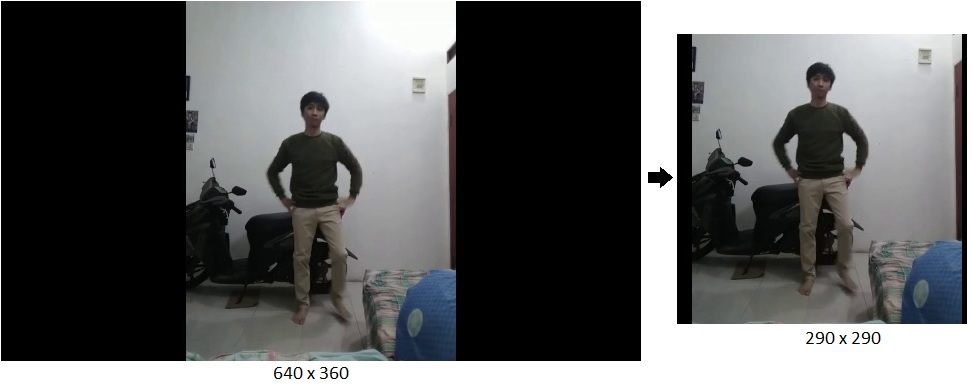
\includegraphics[width=11.9cm]{bab3/gambar/prainferensi.jpg}}
    \end{center}
    \vspace{-20pt}
    \captionsetup{labelfont=bf, textfont=bf}
    \caption{Resolusi Gambar Data Inferensi}
    \vspace{-10pt}
    \captionsetup{labelfont=md, textfont=md}
    % \caption*{Sumber: sumber}
    % \caption*{Sumber: nama(2019)}
    \label{fig:prainferensi}
\end{figure}

\subsection{OpenPose}

OpenPose merupakan aplikasi estimasi pose tubuh manusia dua dimensi. OpenPose menerima input gambar
kemudian mencari titik kunci pose dua dimensi. Titik kunci pose dua dimensi berada pada koordinat
lokal sesuai dengan bidang gambar. OpenPose menghasilkan berkas "json" yang berisi hierarki pose
menurut spesifikasi COCO-MS. Anotasi COCO-MS berisi delapan belas titik kunci tubuh manusia dengan
urutan tertentu seperti
pada gambar ~\ref{fig:coco}. Visualisasi estimasi pose dua dimensi menggunakan OpenPose dapat dilihat
pada gambar~\ref{fig:openpose}.

\begin{figure}[htbp]
    \begin{center}
        \fbox{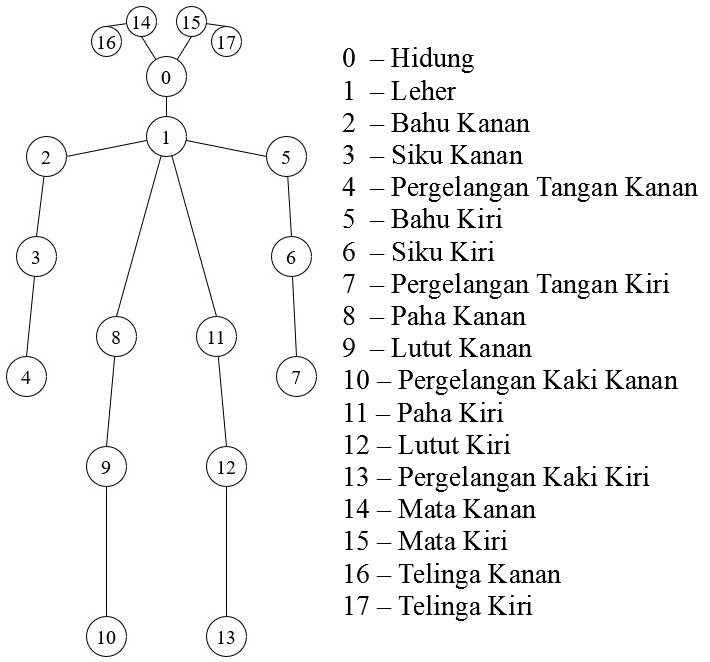
\includegraphics[width=11.9cm]{bab3/gambar/coco.jpg}}
    \end{center}
    \vspace{-20pt}
    \captionsetup{labelfont=bf, textfont=bf}
    \caption{Spesifikasi Titik Kunci COCO-MS}
    \vspace{-10pt}
    \captionsetup{labelfont=md, textfont=md}
    % \caption*{Sumber: sumber}
    % \caption*{Sumber: nama(2019)}
    \label{fig:coco}
\end{figure}


\begin{figure}[htbp]
    \begin{center}
        \fbox{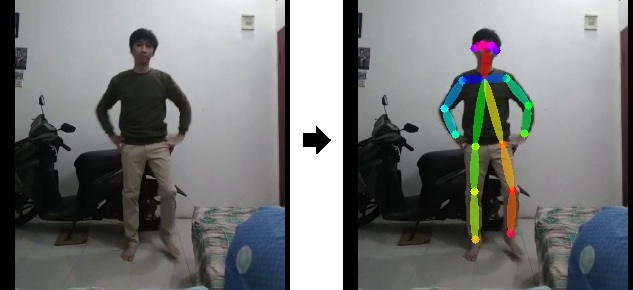
\includegraphics[width=11.9cm]{bab3/gambar/openpose.jpg}}
    \end{center}
    \vspace{-20pt}
    \captionsetup{labelfont=bf, textfont=bf}
    \caption{Inferensi Pose Dua Dimensi OpenPose}
    \vspace{-10pt}
    \captionsetup{labelfont=md, textfont=md}
    % \caption*{Sumber: sumber}
    % \caption*{Sumber: nama(2019)}
    \label{fig:openpose}
\end{figure}

\subsection{Inferensi Model}

Rangkaian titik kunci yang dihasilkan oleh OpenPose memiliki spesifikasi COCO-MS yang berbeda dengan
spesifikasi \textit{dataset} pembuatan model. Spesifikasi COCO-MS yang memiliki delapan belas titik
kunci dikonversi menjadi lima belas titik kunci dengan menyatukan titik kunci kedua mata dan kedua telinga
serta membuat titik kunci pinggang berdasarkan rata-rata kedua kaki bagian atas seperti pada
gambar~\ref{fig:konversi}. Konversi ini dilakukan supaya model dapat melakukan inferensi terhadap
titik kunci yang mewakili pose tersebut. Visualisasi konversi titik kunci COCO-MS menggunakan warna
biru mewakili anggota badan sebelah kanan bersamaan dengan warna merah yang mewakili anggota badan
tengah dan kiri. seperti pada gambar~\ref{fig:konversi_keypoint}.

\begin{figure}[htbp]
    \begin{center}
        \fbox{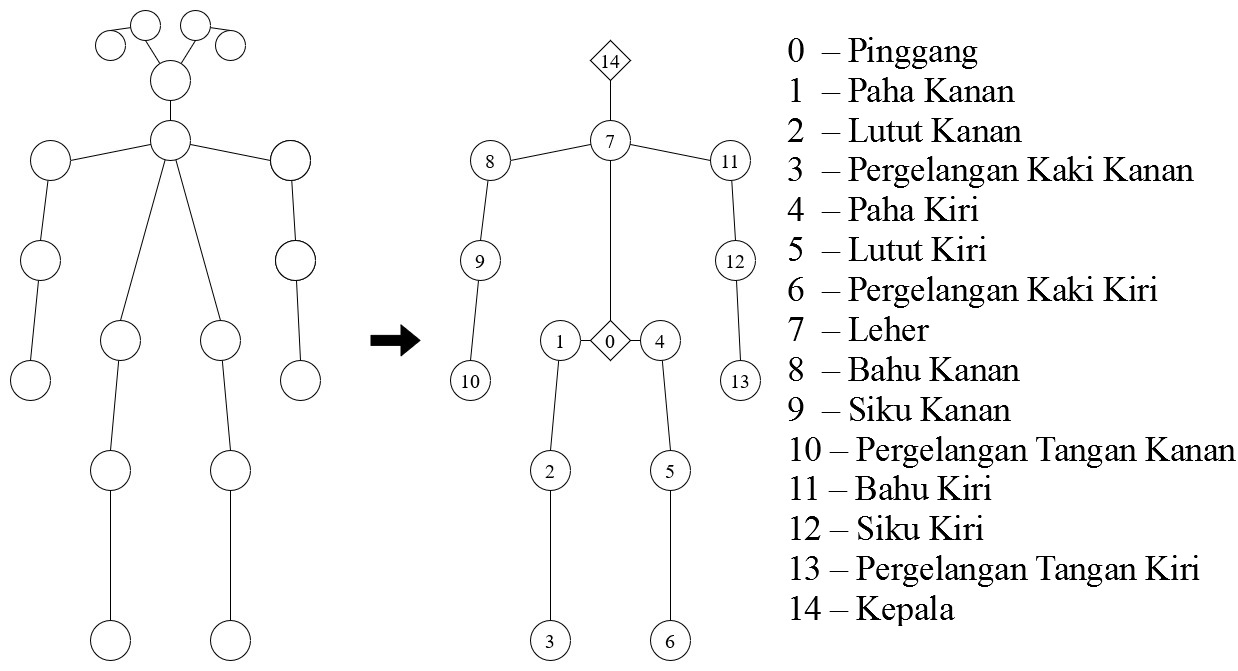
\includegraphics[width=11.9cm]{bab3/gambar/konversi.jpg}}
    \end{center}
    \vspace{-20pt}
    \captionsetup{labelfont=bf, textfont=bf}
    \caption{Konversi Titik Kunci Dua Dimensi}
    \vspace{-10pt}
    \captionsetup{labelfont=md, textfont=md}
    % \caption*{Sumber: sumber}
    % \caption*{Sumber: nama(2019)}
    \label{fig:konversi}
\end{figure}

\begin{figure}[htbp]
    \begin{center}
        \fbox{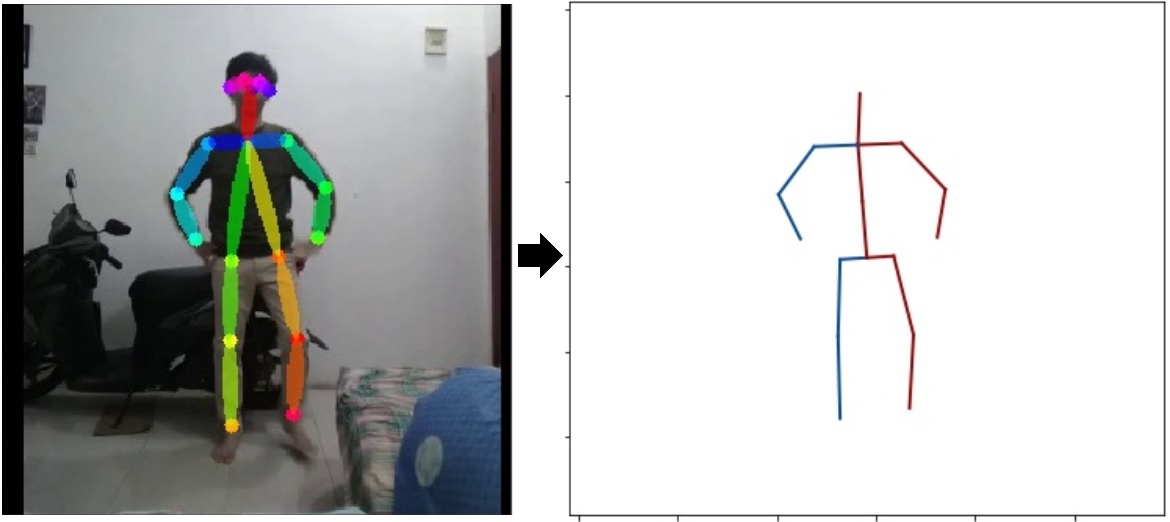
\includegraphics[width=11.9cm]{bab3/gambar/konversi_keypoint.jpg}}
    \end{center}
    \vspace{-20pt}
    \captionsetup{labelfont=bf, textfont=bf}
    \caption{Visualisasi Titik Kunci Dua Dimensi}
    \vspace{-10pt}
    \captionsetup{labelfont=md, textfont=md}
    % \caption*{Sumber: sumber}
    % \caption*{Sumber: nama(2019)}
    \label{fig:konversi_keypoint}
\end{figure}

Inferensi pada model \textit{deep neural network} menerima titik kunci pose dua dimensi yang telah
dikonversi sebagai \textit{input} kemudian menghasilkan titik kunci pose tiga dimensi sebagai \textit{output}.
Inferensi model menghasilkan tujuh belas titik yang berada dalam bidang tiga dimensi.
Titik kunci pose tiga dimensi memiliki dua titik baru yang meliputi torso dan hidung. Titik torso
mewakili lengkungan badan pada pose tiga dimensi sehingga pose terlihat akurat. Titik hidung
mewakili arah hadapan kepala. Kedua titik tambahan ini memperjelas orientasi pose tiga dimensi.
Proses inferensi model untuk mendapatkan pose tiga dimensi dapat
dilihat pada gambar~\ref{fig:inferensi}. Visualisasi inferensi model dapat dilihat pada gambar~\ref{fig:bro118}.

\begin{figure}[htbp]
    \begin{center}
        \fbox{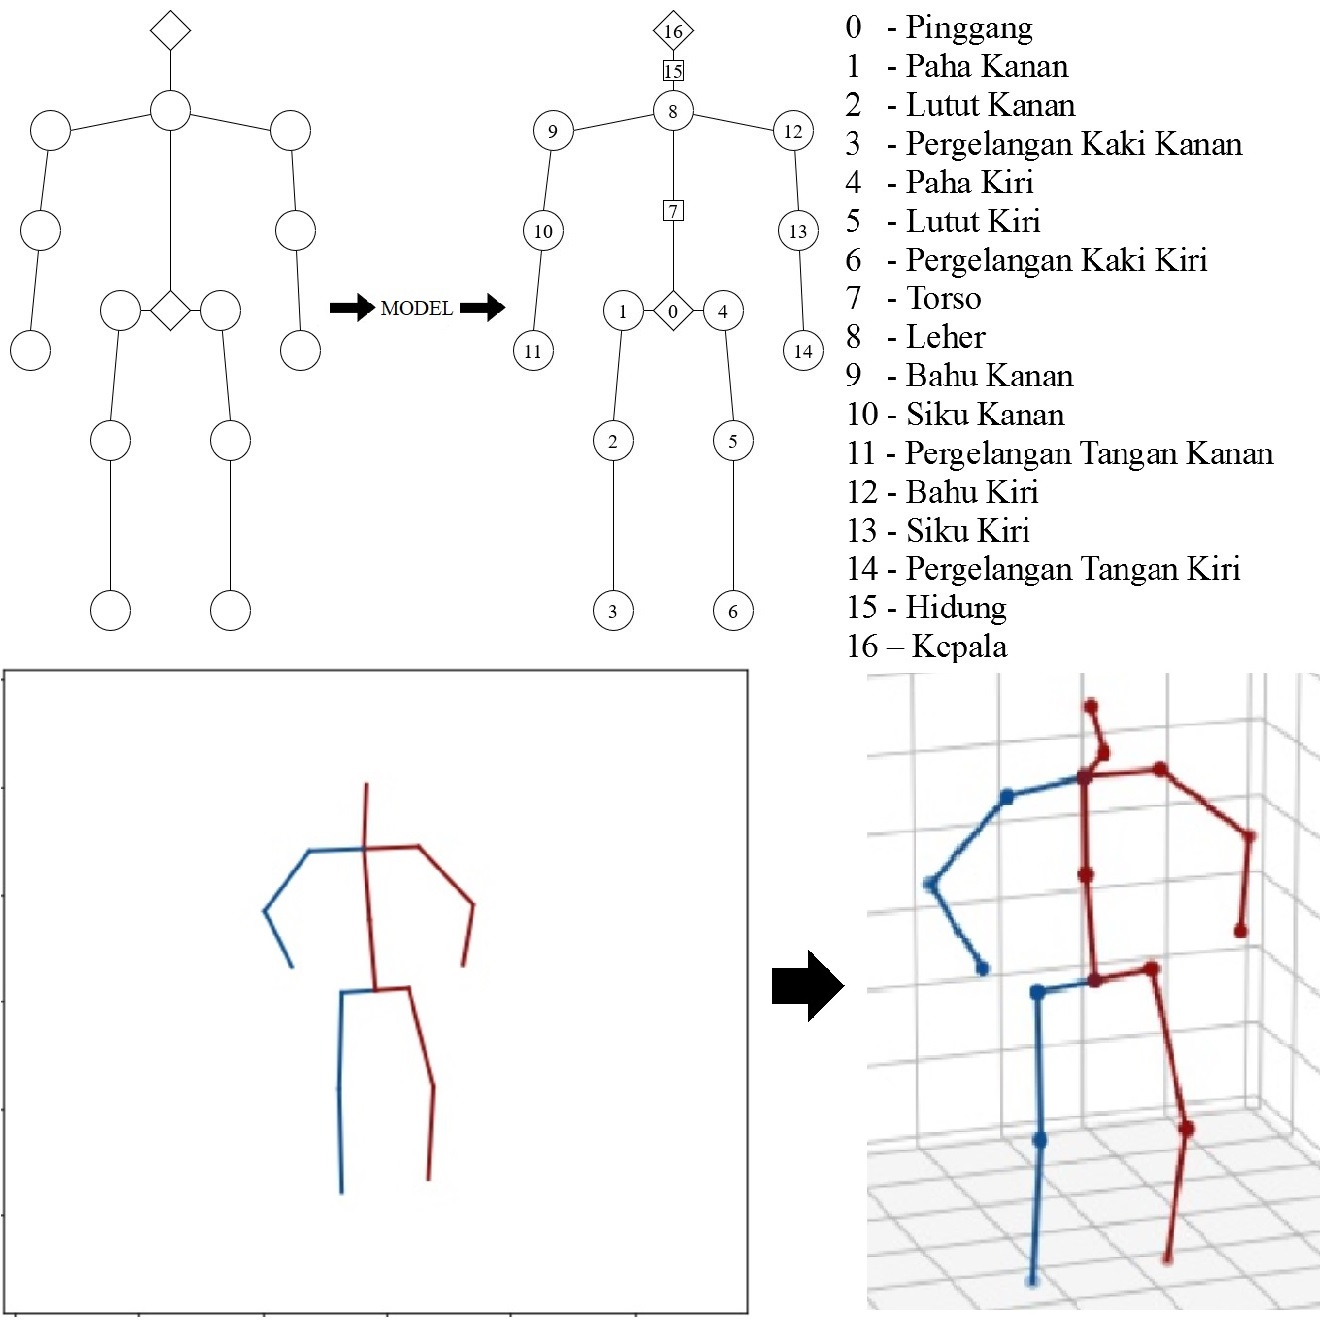
\includegraphics[width=11.9cm]{bab3/gambar/inferensi.jpg}}
    \end{center}
    \vspace{-20pt}
    \captionsetup{labelfont=bf, textfont=bf}
    \caption{Inferensi Model}
    \vspace{-10pt}
    \captionsetup{labelfont=md, textfont=md}
    % \caption*{Sumber: sumber}
    % \caption*{Sumber: nama(2019)}
    \label{fig:inferensi}
\end{figure}

\begin{figure}[htbp]
    \begin{center}
        \fbox{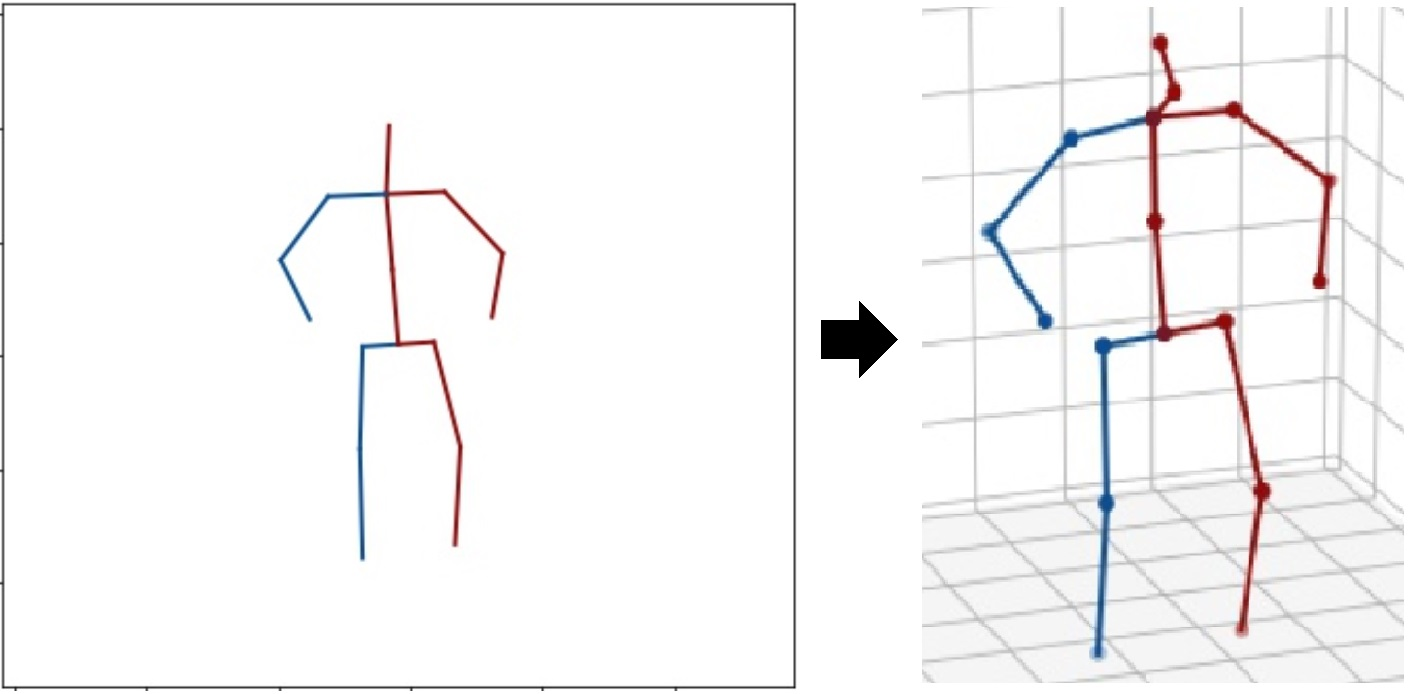
\includegraphics[width=11.9cm]{bab3/gambar/bro118.jpg}}
    \end{center}
    \vspace{-20pt}
    \captionsetup{labelfont=bf, textfont=bf}
    \caption{Visualisasi Titik Kunci Tiga Dimensi}
    \vspace{-10pt}
    \captionsetup{labelfont=md, textfont=md}
    % \caption*{Sumber: sumber}
    % \caption*{Sumber: nama(2019)}
    \label{fig:bro118}
\end{figure}


\subsection{Visualisasi}

Visualisasi mencakup penggunaan aplikasi dalam satu bingkai secara keseluruhan. Terdapat empat buah
figur yang masing-masing mewakili langkah-langkah pada tahapan uji coba. Figur pertama (kiri atas)
berisi prapemrosesan data inferensi dimana resolusi gambar diubah menjadi 290 x 290. Figur kedua
(kanan atas) menggambarkan pose dua dimensi yang didapatkan oleh OpenPose. Figur ketiga (kiri bawah)
menggambarkan konversi titik kunci OpenPose dengan spesifikasi COCO-MS menjadi titik kunci yang cocok
dengan model. Figur keempat (kanan bawah) menggambarkan pose tiga dimensi yang dihasilkan oleh model
kedalam sebuah sistem koordinat tiga dimensi. Contoh visualisasi aplikasi dapat dilihat pada
gambar~\ref{fig:vizapp}.

\begin{figure}[htbp]
    \begin{center}
        \fbox{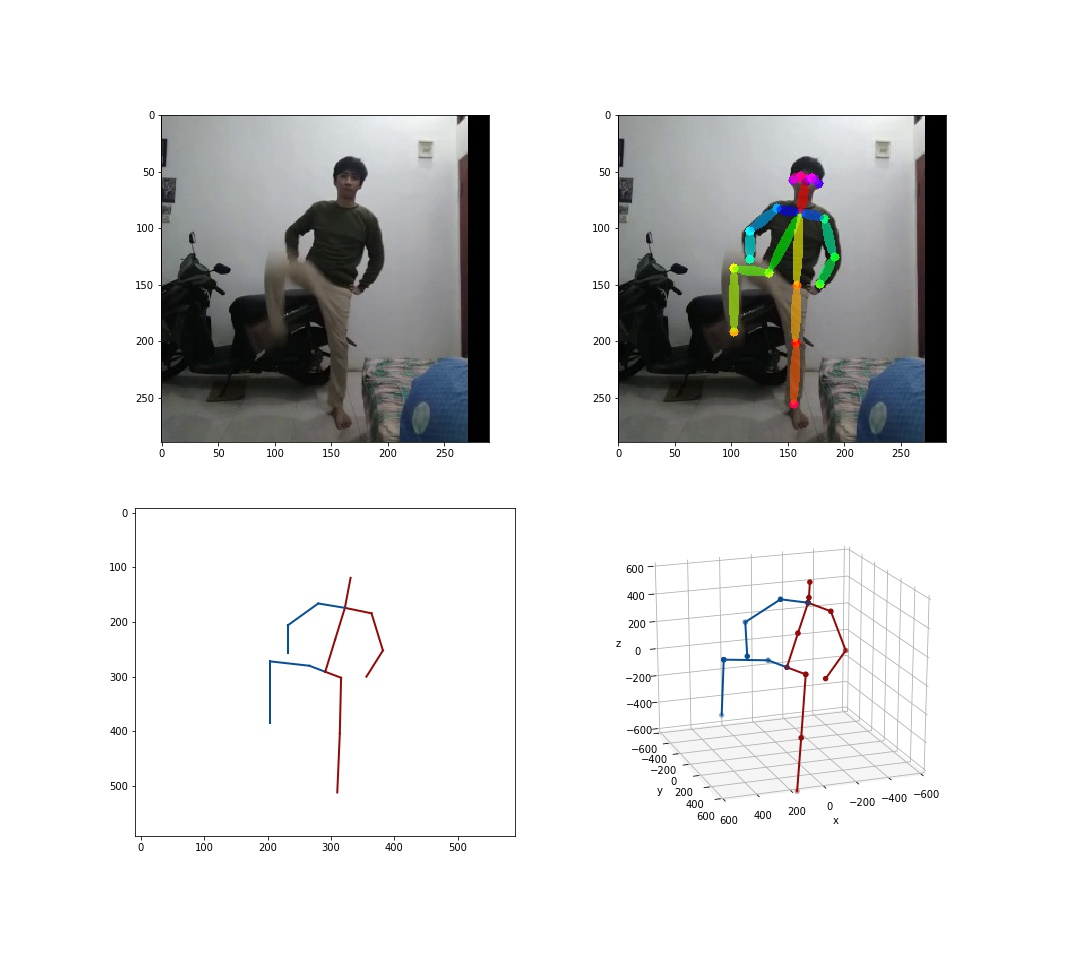
\includegraphics[width=11.9cm]{bab3/gambar/viz135.jpg}}
    \end{center}
    \vspace{-20pt}
    \captionsetup{labelfont=bf, textfont=bf}
    \caption{Visualisasi Aplikasi}
    \vspace{-10pt}
    \captionsetup{labelfont=md, textfont=md}
    % \caption*{Sumber: sumber}
    % \caption*{Sumber: nama(2019)}
    \label{fig:vizapp}
\end{figure}
